\documentclass[11pt]{amsart}
%prepared in AMSLaTeX, under LaTeX2e
\addtolength{\oddsidemargin}{-.65in}
\addtolength{\evensidemargin}{-.65in}
\addtolength{\topmargin}{-0.85in}
\addtolength{\textwidth}{1.4in}
\addtolength{\textheight}{1.3in}
\newcommand{\normalspacing}{\renewcommand{\baselinestretch}{1.03}
        \tiny\normalsize}

\newtheorem*{thm}{Theorem}
\newtheorem*{defn}{Definition}
\newtheorem*{example}{Example}
\newtheorem*{problem}{Problem}
\newtheorem*{remark}{Remark}

\usepackage{amssymb,verbatim,fancyvrb,xspace}
\usepackage{palatino}

\usepackage[final]{graphicx}

\usepackage[pdftex, colorlinks=true, plainpages=false, linkcolor=black, citecolor=red, urlcolor=red]{hyperref}

% macros
\newcommand{\ba}{\mathbf{a}}
\newcommand{\bb}{\mathbf{b}}
\newcommand{\bn}{\mathbf{n}}
\newcommand{\br}{\mathbf{r}}
\newcommand{\bu}{\mathbf{u}}
\newcommand{\bv}{\mathbf{v}}
\newcommand{\bx}{\mathbf{x}}
\newcommand{\by}{\mathbf{y}}

\newcommand{\bT}{\mathbf{T}}

\newcommand{\CC}{\mathbb{C}}
\newcommand{\Div}{\nabla\cdot}
\newcommand{\eps}{\epsilon}
\newcommand{\grad}{\nabla}
\newcommand{\ZZ}{\mathbb{Z}}
\newcommand{\ip}[2]{\ensuremath{\left<#1,#2\right>}}
\newcommand{\lam}{\lambda}
\newcommand{\lap}{\triangle}
\newcommand{\RR}{\mathbb{R}}

\newcommand{\cond}{\operatorname{cond}}

\newcommand{\prob}[1]{\bigskip\noindent\textbf{#1}\, }
\newcommand{\ppart}[1]{\textbf{(#1)}\,\, }
\newcommand{\epart}[1]{\medskip\noindent\textbf{(#1)}\,\, }

\newcommand{\pts}[1]{\scriptsize [#1 points] \normalsize}

\newcommand{\Matlab}{\textsc{Matlab}\xspace}
\newcommand{\Octave}{\textsc{Octave}\xspace}
\newcommand{\Python}{\textsc{Python}\xspace}

\newcommand{\mfile}[2]{
	\medskip
	\begin{quote}
		\bigskip
		\VerbatimInput[frame=single,framesep=3mm,label=\fbox{\normalsize \textsl{\,#1\,}},fontfamily=courier,fontsize=\scriptsize]{#2}
		\bigskip
	\end{quote}
}

\DefineVerbatimEnvironment{mVerb}{Verbatim}{numbersep=2mm,frame=lines,framerule=0.1mm,framesep=2mm,xleftmargin=4mm,fontsize=\footnotesize}



\begin{document}
\scriptsize \phantom{bob} \vspace{-0.3in}
\noindent Math 615 Numerical Analysis of Differential Equations \, (Bueler) \hfill  \today
\normalsize\bigskip
\normalspacing

\Large\centerline{\textbf{Worksheet solutions}}
\normalsize

\bigskip\medskip
\thispagestyle{empty}
\normalspacing


\prob{TASK (a)}  I computed stability functions for the first two methods:
\begin{align*}
R_{\text{TR}}(z) &= \frac{1+z/2}{1-z/2}, \\
R_{\text{RK2}}(z) &= 1 + z + \frac{z^2}{2}.
\end{align*}
The stability regions are $S = \{z\in\CC\,:\,|R(z)|\le 1\}$.  For AB2 FIXME

FIXME I wrote the following code which generates Figure 1:

\mfile{regions.m}{regions.m}

Nontrivial quantitative results to note are that on the real axis RK2 has a stability interval $[-2,0]$ while BDF2 is not absolutely stable on the interval $[0,4]$.

\begin{figure}[b]
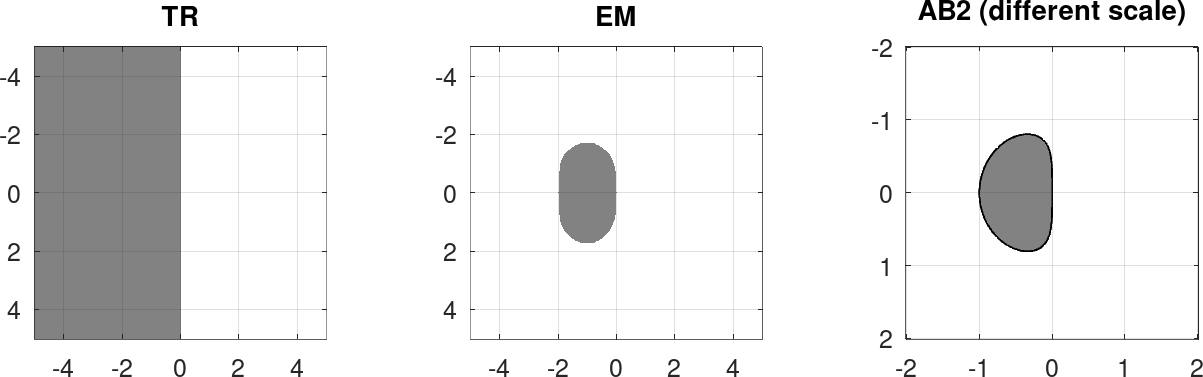
\includegraphics[width=0.7\textwidth]{regions.pdf}
\caption{Stability regions generated by \texttt{regions.m}.}
\label{fig:regions}
\end{figure}

\prob{TASK b)}  FIXME Note that the S1 and S3 matrices are symmetric, so the eigenvalues are real in those cases.  I wrote the following easy code to get the eigenvalues:

\mfile{alleigens.m}{/home/ed/repos/bueler.github.io/M615S17/matlab/alleigens.m}

Here is the result, with slightly-improved formatting:
\begin{mVerb}
>> alleigens
S1:
  -5.56551  -0.52687  4.09237
S2:
  0.00000 - 2.00000i  0.00000 + 2.00000i
S3:
  -2694.14240  -2664.71334  -2616.14196  -2549.13655  -2464.67419  -2363.98653
  -2248.54183  -2120.02354  -1980.30573  -1831.42581  -1675.55478  -1514.96559
  -1352.00000  -1189.03441  -1028.44522   -872.57419   -723.69427   -583.97646
   -455.45817   -340.01347   -239.32581   -154.86345    -87.85804    -39.28666
     -9.85760
\end{mVerb}
In particular, S1 has two negative and one positive eigenvalue, both eigenvalues in S2 are purely imaginary, and S3 has only negative eigenvalues.

\prob{TASK c)}  The main idea is that

\begin{quote}
\emph{For those eigenvalues $\lambda$ that have negative real parts, corresponding to decaying components of an exact solution, absolute stability ``$|U^{n+1}|\le |U^n|$'' is a useful requirement in choosing the time-step.  Thus we choose the largest $k_{\text{stab}}$ so that}
    $$z = k_{\text{stab}} \lambda$$
\emph{is in the region of absolute stability for all $\lambda$ such that $\operatorname{Re}(\lambda)<0$, and we only use time steps $k$ such that $k\le k_{\text{stab}}$.}
\end{quote}

For the negative eigenvalues in problem S1, absolute stability is relevant.  The problem also has one positive eigenvalue, and generally absolute stability might not be useful for it, but we would probably want BDF2 to \emph{not} satisfy ``$|U^{n+1}|\le |U^n|$'', so we can think of that as a stability restriction.

Since S2 has only purely-imaginary eigenvalues, I conclude that absolute stability has nothing to say about it, regardless of the method.

For S3, all eigenvalues are negative so both TR and BDF2 have no stability restrictions but the stability restriction for RK2 is severe.

\clearpage
\newpage

I put my results in a table:

\bigskip
\begin{center}
\begin{tabular}{r|c|c|c}
   & \phantom{sdljf} TR \phantom{sdljf} & \phantom{sdljf} RK2 \phantom{sdljf} & \phantom{sdljf} BDF2 \phantom{sdljf} \\ \hline
S1 & $\ast$ & $k_{\text{stab}} = 0.360$ & $k_{\text{stab}} \stackrel{?}{=} 0.977$\\ \hline
S2 & $\dagger$ & $\dagger$ & $\dagger$ \\ \hline
S3 & $\ast$ & $k_{\text{stab}} = 0.000742$ & $\ast$
\end{tabular}
\end{center}

\bigskip
There are these cases to explain:
\begin{itemize}
\item[$\ast$:]     These implicit methods have \emph{no stability restriction} because decaying eigenvalues give decaying approximate solutions, and growing give growing.
\item[$\dagger$:]  Since all eigenvalues of S2 have nonnegative real parts (i.e.~zero real parts), there are \emph{no stability restrictions}.
\item[?:]          In this case we might restrict the step this way so that the positive eigenvalue corresponds to a growing approximate solution.
\end{itemize}

\prob{TASK d)}  My expert advice:

\begin{itemize}
\item[S1:] I would recommend using RK2 subject to the given stability restriction.  (One would usually choose time steps much smaller than 0.360 anyway, but for accuracy.)  The reason to choose this method is ease of implementation and low computational cost, as it is an explicit method.
\item[S2:] Any of the methods are probably o.k.~for any step size which is small enough to give decent accuracy.  But note that the eigenvalues $\lambda=\pm 2 i$ correspond to exact solution components which are purely-oscillating, with neither decay nor growth.  Because these eigenvalues correspond to points $z$ which are on the exact boundary of its stability region, method TR has the interesting property that it generates approximate solutions which also neither decay nor grow.  I would choose TR given that it is not too hard to implement on a linear problem like this.  (\emph{An observation like this explains why TR is standard for the Sch\"odinger equation: it preserves unitarity.})
\item[S3:] I would choose either TR or BDF2 because the stability restriction for RK2 is severe and stops us from doing long time steps.  (\emph{That is, even if a long time step would be acceptable accuracy-wise.})  We will see that for smooth initial data both TR and BDF2 work well on discretized heat equations for essentially any time step.  But if the initial condition is rough then for large time steps TR will have worse-looking results because it does not kill off the high frequencies as it should; it is common to choose BDF2 for problems like the heat equation with rough data.  (\emph{In Chapter 8 we see that a simple modification of BDF2 is L-stable, and this is one way to state the desired good behavior for rough data.})
\end{itemize}

\end{document}
